\section{Graph}

\vspace{\parskip}

\begin{definition}[Undirected Graph] \index{undirected graph}
    An undirected graph is the ordered pair $G=(V,E)$ where $V$ is the set of nodes/vertices, and $E$ is the set of edges defined by $E \subseteq \{ \{u,v\} \mid u,v \in V,\, u \neq v \}$.
\end{definition}

\begin{definition}[Directed Graph] \index{directed graph}
    A directed graph is the ordered pair $G=(V,E)$ where $E$ is the set of ordered pairs $E \subseteq V \times V$.
\end{definition}

We use $n = |V|$ to denote the number of vertices, and $m = |E|$ to denote the number of edges in a graph. For an undirected graph, $|E| \leq \choose{n 2}$ and $|E| \leq n^2$ for directed graph. 

\begin{definition}[Neighbors and Degrees] \index{neighbors} \index{predecessor} \index{successor} \index{degree} \index{in-degree} \index{out-degree}
    For any edge $uv$ in an undirected graph, we call $u$ neighbor of $v$ and vice versa, and we say that $u$ and $v$ are adjacent. The degree of a node is its number of neighbors.

    In directed graphs, for every edge $u \to v$, we call $u$ a predecessor of $v$, and we call $v$ a successor of $u$. The in-degree of a vertex is its number of predecessors; the out-degree is its number of sucessors.
\end{definition}

\begin{definition}[Subgraphs] \index{subgraphs}
    A graph $G' = (V',E')$ is a subgraph of $G=(V,E)$ if $V' \subseteq V$ and $E' \subseteq E$. A proper subgraph of $G$ is any subgraph that is not $G$ itself.
\end{definition}


\subsection{Other Types of Graphs} \index{simple graph} \index{hypergraph} \index{weighted graph}

A \textbf{simple graph} has no multiple edges or self loops.

A \textbf{hypergraph} is a graph consists of vertices and hyperedges. A hyperedge is a nonempty set of vertices.

A \textbf{weighted graph} has a weight function $w:\; E \to \R$ that assign a weight to each edge. We can similarly define a weight function for the vertices.

An \textbf{subgraph} $G'$ of $G$ \textbf{induced} by $V'$ is the graph $(V',E')$ such that $E' = \{ \{u,v\} \in E \mid u,v \in V' \}$. 

\section{Operations on Graphs}

\begin{multicols}{2}
    \begin{itemize}
        \item Find the shortest path between $u,v\in V$.
        \item Cycle detection.
        \item Compute degree of a vertex ($\mathrm{deg}(v)$ is the number of neighbors of a vertex).
        \item Add/Delete vertices.
        \item Add/Delete edges.
        \item Check if there is a path between $u$ and $v$.
        \item Topological sort of a directed acyclic graph (DAG)
        \item Find a clique (a set of nodes $C$ such that $\forall u,v \in C.\, u \neq v,\, \{u,v\} \in E$)
        \item Color a graph.
        \item Find minimal spanning tree.
        \item Find all nodes $u$ that are connected to some node $v$.
        \item Find all neighbors of $v$.
        \item Find all connected components in an undirected graph.
        \item Check if $G$ is induced subgraph.
        \item Find maximal matching.
        \item Check isomorphism.
        \item Compute flows (minimum and maximum flow) in a weighted directed graph.
    \end{itemize}
\end{multicols}

\section{Data Structures for Representing Graph}

\subsection{List of Edges}

We can simply store a graph as a list of all edges in the graph. It takes $O(m)$ words, each of $O(\lg n)$ bits. The list can either be sorted or unsorted.

\subsection{Adjacency Matrix} \index{adjacency matrix}

\vspace{\parskip}

\begin{definition}[Adjacency Matrix]
    An adjacency matrix is a matrix whose rows and columns are indexed by $V$ where $A[u,v]=1$ if and only if $\{u,v\} \in E$ for undirected graph or $(u,v) \in E$ for directed graph.
\end{definition}

This representation takes $O(n^2)$ space. It is efficient if the grraph is dense (i.e. $m \in \Omega(n^2)$).

\subsection{Adjacency List}

\vspace{\parskip}

\begin{definition}[Adjacency List] \index{adjacency list}
    The adjacency-list representation of a graph $G=(V,E)$ consists of an arrray \textit{Adj} of $|V|$ lists, one for each vertex in $V$. For each $u \in V$, the adjacency list \textit{Adj[u]} contains all the vertices $v$ such that there is an edge $(u,v) \in E$. That is, \textit{Adj}[u] contains all the vertices adjacent to $u$ in $G$.
\end{definition}

It requires $O(n+m)$ words to store an adjacency list. There are in total $2m$ entries in these lists, and each word is $O(\lg n)$ bits. This representation is efficient if the graph is sparse (i.e. $m \in O(n)$ or $m \in O(n \log n)$).

\begin{figure}[htbp]
    \centering
    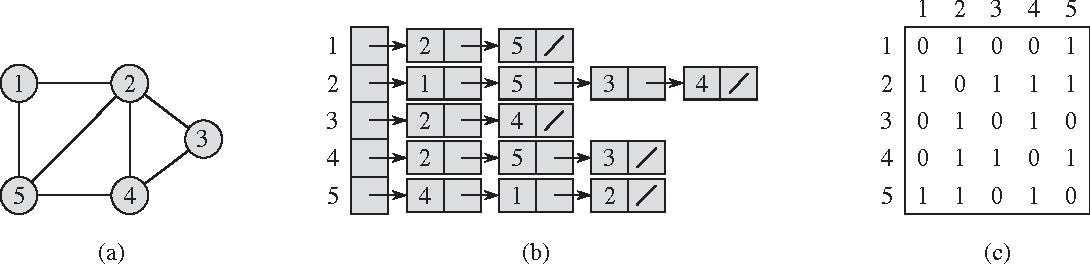
\includegraphics[width=\linewidth]{figures/undirected_graph.pdf}
    \caption{Representations of undirected graph: (a) the graph; (b) adjacency list of the graph; (c) adjacency matrix of the graph.}
    \label{fig:graph-rep}
\end{figure}

\section{Incidence Matrix} \index{incidence matrix}

$M[v,e]=0$ if $v$ is not incident to $e$. For undirected graph, $M[v,e]=1$ if $v$ is incident to $e$. For directed graph, $M[v,e]=1$ if $v$ is the destination of $e$ and $-1$ if $v$ is the source of $e$. A self-loop is typically represented using a special value.

We can store the weight in the matrix if $w(v) \in \R^+$. 

\section{Time Complexity}

The time complexity of operations depend on the representation. For example, consider the problem of checking whether or not $\{u,v\} \in E$.

\begin{itemize}
    \item Adjacency matrix: $O(1)$
    \item Adjacency list: $O(n)$ or $O(\mathrm{deg}(u))$
    \item List of edges: $O(m)$ or $O(\log n)$
    \item Incidence matrix: $O(m)$  
\end{itemize}

For the problem of finding the neighbors

\begin{itemize}
    \item Adjacency matrix: $O(n)$ 
    \item Adjacency list: $O(1)$ 
    \item List of edges: $O(m)$ 
    \item Incidence matri: $O(m)$ 
\end{itemize}


\begin{theorem}[Rivest-Vuiellemin Theorem] \index{Rivest-Vuiellemin Theorem}
    Any nontrivial monotone graph property that is invariant under isomorphism requires $\Omega(n^2)$ adjacency matrix probes. Monotone means the property does not change from True to False when more edges are added.
\end{theorem}